\documentclass{article}

\newif\ifanswers
\answerstrue % comment out to hide answers

\usepackage{fancyhdr} % Required for custom headers
\usepackage{lastpage} % Required to determine the last page for the footer
\usepackage{extramarks} % Required for headers and footers
\usepackage[usenames,dvipsnames]{color} % Required for custom colors
\usepackage{graphicx} % Required to insert images
\usepackage{listings} % Required for insertion of code
\usepackage{courier} % Required for the courier font
\usepackage{lipsum} % Used for inserting dummy 'Lorem ipsum' text into the template
\usepackage{enumerate}
\usepackage{enumitem}
\usepackage{booktabs}
\usepackage{amsmath, amsthm, amssymb}
\usepackage[margin=1cm]{caption}
\usepackage{subcaption}
\captionsetup[table]{skip=4pt}
\usepackage{framed}
\usepackage{bm}
\usepackage[most]{tcolorbox}
\usepackage[colorlinks]{hyperref}
\usepackage{hyperref}
\usepackage{float}


% guillaume edits
\usepackage{xcolor}
\graphicspath{{img/}} % set of paths to search for images
\usepackage{amsmath}
\usepackage{amsfonts}
\usepackage{amssymb}

\newenvironment{myitemize}
{ \begin{itemize}
		\setlength{\itemsep}{0pt}
		\setlength{\parskip}{0pt}
		\setlength{\parsep}{0pt}     }
	{ \end{itemize}                  } 
% end guillaume edits

\usepackage{biblatex} % bibliography
\addbibresource{papers.bib}

\usepackage{tikz}
\usetikzlibrary{positioning,patterns,fit}

\newcommand{\ifans}[1]{\ifanswers \color{red} \textbf{Solution: } #1 \color{black}}

% Margins
\topmargin=-0.45in
\evensidemargin=0in
\oddsidemargin=0in
\textwidth=6.5in
\textheight=9.0in
\headsep=0.25in

\linespread{1.1} % Line spacing

% Set up the header and footer
\pagestyle{fancy}
\rhead{\hmwkAuthorName} % Top left header
\lhead{\hmwkClass: \hmwkTitle} % Top center head
\lfoot{\lastxmark} % Bottom left footer
\cfoot{} % Bottom center footer
\rfoot{Page\ \thepage\ of\ \protect\pageref{LastPage}} % Bottom right footer
\renewcommand\headrulewidth{0.4pt} % Size of the header rule
\renewcommand\footrulewidth{0.4pt} % Size of the footer rule

\setlength\parindent{0pt} % Removes all indentation from paragraphs

%----------------------------------------------------------------------------------------
%	CODE INCLUSION CONFIGURATION
%----------------------------------------------------------------------------------------

\DeclareMathOperator*{\argmin}{arg\,min}
\DeclareMathOperator*{\argmax}{arg\,max}
\newcommand{\prob}{\mathbb P}
\newcommand{\Var}{\mathbb V}
\newcommand{\Ex}{\mathbb E}



\definecolor{MyDarkGreen}{rgb}{0.0,0.4,0.0} % This is the color used for comments
\lstloadlanguages{Python} % Load Perl syntax for listings, for a list of other languages supported see: ftp://ftp.tex.ac.uk/tex-archive/macros/latex/contrib/listings/listings.pdf
\lstset{language=Python, % Use Perl in this example
        frame=single, % Single frame around code
        basicstyle=\footnotesize\ttfamily, % Use small true type font
        keywordstyle=[1]\color{Blue}\bf, % Perl functions bold and blue
        keywordstyle=[2]\color{Purple}, % Perl function arguments purple
        keywordstyle=[3]\color{Blue}\underbar, % Custom functions underlined and blue
        identifierstyle=, % Nothing special about identifiers
        commentstyle=\usefont{T1}{pcr}{m}{sl}\color{MyDarkGreen}\small, % Comments small dark green courier font
        stringstyle=\color{Purple}, % Strings are purple
        showstringspaces=false, % Don't put marks in string spaces
        tabsize=5, % 5 spaces per tab
        %
        % Put standard Perl functions not included in the default language here
        morekeywords={rand},
        %
        % Put Perl function parameters here
        morekeywords=[2]{on, off, interp},
        %
        % Put user defined functions here
        morekeywords=[3]{test},
       	%
        morecomment=[l][\color{Blue}]{...}, % Line continuation (...) like blue comment
        numbers=left, % Line numbers on left
        firstnumber=1, % Line numbers start with line 1
        numberstyle=\tiny\color{Blue}, % Line numbers are blue and small
        stepnumber=5 % Line numbers go in steps of 5
}

% Creates a new command to include a perl script, the first parameter is the filename of the script (without .pl), the second parameter is the caption
\newcommand{\perlscript}[2]{
\begin{itemize}
\item[]\lstinputlisting[caption=#2,label=#1]{#1.pl}
\end{itemize}
}

%----------------------------------------------------------------------------------------
%	NAME AND CLASS SECTION
%----------------------------------------------------------------------------------------

\newcommand{\hmwkTitle}{Assignment \#3} % Assignment title
\newcommand{\hmwkClass}{CS\ 234} % Course/class
\newcommand{\hmwkAuthorName}{} % Your name

%----------------------------------------------------------------------------------------
%	TITLE PAGE
%----------------------------------------------------------------------------------------

\title{
\vspace{-1in}
\textmd{\textbf{\hmwkClass:\ \hmwkTitle\\
Winter 2019}}}
\author{ Li Quan Khoo (SCPD) }
\date{} % Insert date here if you want it to appear below your name

\begin{document}

\maketitle
\vspace{-.5in}


\section{Policy Gradient Methods (50 pts + 15 pts writeup)}

\subsection{Coding Questions (50 pts)}
\begin{itemize}
\item \url{https://github.com/lqkhoo/cs234-winter-2019/blob/master/assignment3/pg.py}
\end{itemize} 

\subsection{Writeup Questions (15 pts)}
\begin{enumerate}
\item[(a) (4 pts)] (CartPole-v0)
\begin{figure}[H]
	\centering
	\begin{subfigure}[b]{.4\textwidth}
		\centering
		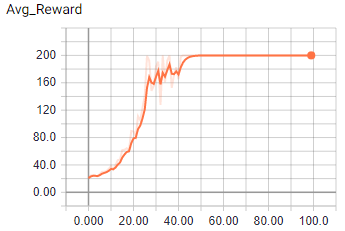
\includegraphics[width=0.9\linewidth]{cartpole-baseline-avgreward.png}
		\caption{CartPole-v0 with baseline. Average reward over 100 iterations.}
	\end{subfigure}
	\qquad
	\begin{subfigure}[b]{.4\textwidth}
		\centering
		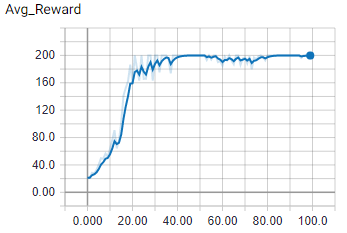
\includegraphics[width=0.9\linewidth]{cartpole-nobaseline-avgreward.png}
		\caption{CartPole-v0 without baseline. Average reward over 100 iterations.}
	\end{subfigure}
\end{figure}

Where
\begin{align*}
r(\tau) = \sum_{t}^{} r(s_t, a_t), \quad and \quad J(\theta) = \Ex_{\tau \sim P_{\theta}(\tau)}[r(\tau)],
\end{align*}
We have derived the Monte-Carlo estimate of the gradient of $J(\theta)$ for policy gradient to be:
\begin{align*}
\nabla_{\theta} J(\theta) &\approx \frac{1}{N}\sum_{i=1}^{N}\nabla_{\theta}log\pi_{\theta}(\tau)[r(\tau)-b]
\end{align*}

Where $b$ is some constant scalar bias of the reward function. Mathematically, the baseline is just another bias, and we already know that this gradient $\nabla_{\theta}J(\theta)$ is indifferent to the bias \textit{in expectation}. However, the actual size and value of the bias still influences convergence (consider a bias close to +/- infinity) due to how the probability mass of the policy is shifted when we perform the gradient update, as well as the variance of the quantity $r(\tau)-b$. (Berkeley CS294, lecture 4)

Here, the baseline we are taking is the state value function $V(s_t)$, which represents the average of returns of all actions from that state. Suppose we have a good estimate of $V(s_t)$. Mathematically, $V(s_t)$ already summarizes all future returns, and the advantage $A(s_t, a_t) = r(s_t, a_t) - V(s_t)$ becomes insulated from the variance of returns of all future time steps \textit{in the current trajectory}. This lowers the variance of our estimated action values. Semantically, we are shifting the probability mass of the policy to make actions which are \textit{better than average} (our chosen baseline) to be more likely.

Empirically, we can see from the plots above that using the baseline tends to give "better" convergence, although this is far from being guaranteed. Our observation here is that the plateau is more stable. The standard deviation of rewards (not shown here) tends to be lower as well.

\item[(b) (4 pts)](InvertedPendulum-v1)

\begin{figure}[H]
	\centering
	\begin{subfigure}[b]{.4\textwidth}
		\centering
		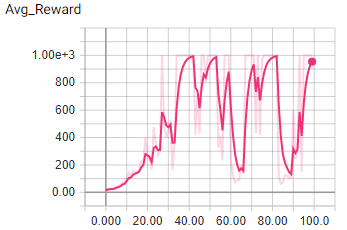
\includegraphics[width=0.9\linewidth]{pendulum-baseline-avgreward.png}
		\caption{Pendulum-v1 with baseline. Average reward over 100 iterations.}
	\end{subfigure}
	\qquad
	\begin{subfigure}[b]{.4\textwidth}
		\centering
		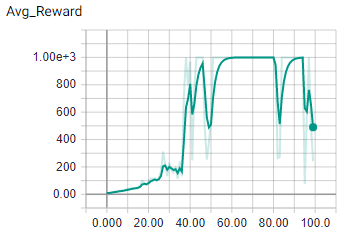
\includegraphics[width=0.9\linewidth]{pendulum-nobaseline-avgreward.png}
		\caption{Pendulum-v1 without baseline. Average reward over 100 iterations.}
	\end{subfigure}
\end{figure}

In this case, we notice that running with baseline tends to have faster convergence, but here, it doesn't seem to help very much with the instability of the algorithm. This instability is due to the high variance of REINFORCE (Monte-Carlo "vanilla" policy gradient), relative to comparable methods such as natural policy gradient and TRPO.

\item[(c) (7 pts)](HalfCheetah-v1)

\begin{figure}[H]
	\centering
	\begin{subfigure}[b]{.4\textwidth}
		\centering
		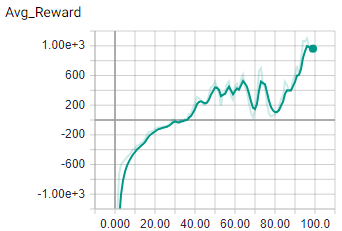
\includegraphics[width=0.9\linewidth]{cheetah-baseline-avgreward.png}
		\caption{HalfCheetah-v1 with baseline. Average reward over 100 iterations.}
	\end{subfigure}
	\qquad
	\begin{subfigure}[b]{.4\textwidth}
		\centering
		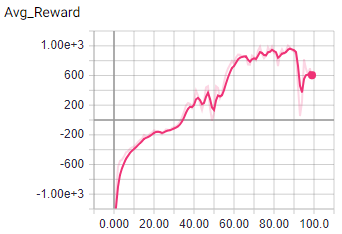
\includegraphics[width=0.9\linewidth]{cheetah-nobaseline-avgreward.png}
		\caption{HalfCheetah-v1 without baseline. Average reward over 100 iterations.}
	\end{subfigure}
\end{figure}

In this particular run, the baseline didn't seem to help, although on average it's supposed to have the same properties as explained in (a) by reducing the variance of the gradient.

\end{enumerate}
 \newpage

\section{Best Arm Identification in Multiarmed Bandit (35pts)}
In this problem we focus on the Bandit setting with rewards bounded in $[0,1]$. A Bandit problem instance is defined as an MDP with just one state and action set $\mathcal A$. Since there is only one state, a ``policy'' consists of the choice of a single action: there are exactly $A = |\mathcal A|$ different deterministic policies. Your goal is to design a simple algorithm to identify a near-optimal arm with high probability.

Imagine we have $n$ samples of a random variable $x$, $\{x_1, \dots, x_n\}$. We recall Hoeffding's inequality below, where $\overline x$ is the expected value of a random variable $x$, $\widehat x= \frac{1}{n} \sum_{i=1}^n x_i$ is the sample mean (under the assumption that the random variables are in the interval [0,1]), $n$ is the number of samples  and $\delta >0$ is a scalar:

\begin{align*}
\Pr\Bigg(|\widehat x - \overline x | > \sqrt{\frac{\log(2/\delta)}{2n}}	\Bigg) < \delta.
\end{align*}

Assuming that the rewards are bounded in $[0,1]$,
we propose this simple strategy: allocate an identical number of samples $n_1 = n_2=...=n_{A} = n_{des}$ to every action, compute the average reward (empirical payout) of each arm $\widehat r_{a_1}, \dots, \widehat r_{a_A}$ and return the action with the highest empirical payout $\arg\max_a \widehat r_{a}$. The purpose of this exercise is to study the number of samples required to output an arm that is at least $\epsilon$-optimal with high probability.
Intuitively, as $n_{des}$ increases the empirical payout $\widehat r_a$ converges to its expected value $\overline r_a$ for every action $a$, and so choosing the arm with the highest empirical payout $\widehat r_a$ corresponds to approximately choosing the arm with the highest expected payout $\overline r_a$.

\begin{enumerate}

\item[(a) (15 pts)] We start by defining a \emph{good event}. Under this \emph{good event}, the empirical payout of each arm is not too far from its expected value. Starting from Hoeffding inequality with $n_{des}$ samples allocated to every action show that:

\begin{align*}
\Pr\Bigg(\exists a \in \mathcal A \quad s.t. \quad |\widehat r_a - \overline r_a | > \sqrt{\frac{\log(2/\delta)}{2n_{des}}}	\Bigg) < A\delta.
\end{align*}

In other words, the \emph{bad event} is that at least one arm has an empirical mean that differs significantly from its expected value and this has probability at most $A\delta$.

\item[(b) (20 pts)] After pulling each arm (action) $n_{des}$ times our algorithm returns the arm with the highest empirical payout:
\begin{equation*}
a^\dagger = argmax_{a} \widehat r_a	
\end{equation*}
Notice that $a^\dagger$ is a random variable.
 Define ${a^\star}$ as the optimal arm (that yields the highest average reward ${a^\star} = argmax_a \overline r_{a}$). Suppose that we want our algorithm to return at least an $\epsilon$ optimal arm with probability $1-\delta'$, as follows:

\begin{equation*}
	\Pr \Bigg(\overline r_{a^\dagger} \geq  \overline r_{a^\star} - \epsilon \Bigg) \geq 1-\delta'.
\end{equation*}
How many samples are needed to ensure this? Express your result as a function of the number of actions $A$, the required precision $\epsilon$ and the failure probability $\delta'$.

\end{enumerate}

\printbibliography



\end{document}
